\subsection{Prototypical Networks for Few Shot Learning}

Prototypical networks is a proposal for the problem of few-shot classification, where a classifier must generalize to new classes not seen in the training set, given only a small number of examples of each new class. The ability of a algorithm to perform few-shot learning is typically measured by its performance on n-shot, k-way classification tasks. First a model is given a query sample belonging to a new, previously unseen class. Then, it’s also given a support set, S, consisting of n examples, each from k different unseen classes. Finally, the algorithm then has to determinate which of the support set classes the query samples belong to.

\begin{figure}[H]
    \centering
        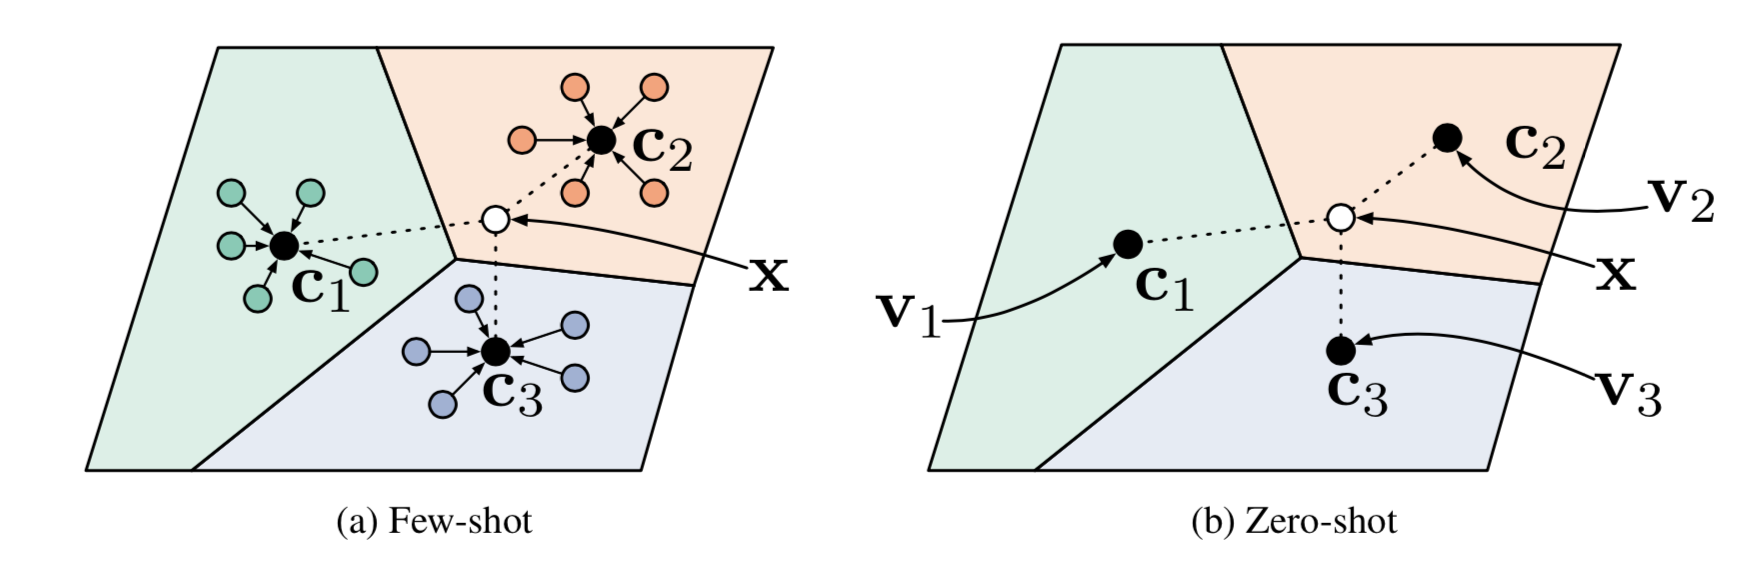
\includegraphics[width=0.8\textwidth]{background/prototypical-networks.png}
    \caption{Figure (1) of the paper. Prototypical networks in the few-shot and zero-shot scenarios. \textbf{Left}: Few-shot prototypes $c_k$ are computed as the mean of embedded support examples for each class. \textbf{Right}: Zero-shot prototypes $c_k$ are produced by embedding class meta-data $v_k$. In either case, embedded query points are classified via a softmax over distances to class prototypes: \\ $p_{\phi}(y = k|x)$ $\alpha$ $e^{−d(f_{\phi}(x), c_k)}$.}
    \label{figure:background:prototypical}
\end{figure}

In Prototypical Networks \cite{protonet} Snell et al. apply a compelling inductive bias in the form of class prototypes to achieve impressive few-shot performance, exceeding Matching Networks \cite{matchingnet} without the complication of FCE. The key assumption is made is that there exists an embedding in which samples from each class cluster around a single prototypical representation which is simply the mean of the individual samples. This idea streamlines n-shot classification in the case of $n > 1$ as classification is simply performed by taking the label of the closest class prototype.

\begin{equation}
    c_k = \frac{1}{|S_k|} \sum_{(\mathbf{x}_i, y_i) \in S_k} f_{\phi}(\mathbf{x}_i)
\end{equation}
\captionof{figure}{Equation (1) from Prototypical Network calculating class prototypes. $S_k$ is the support set belonging to class $k$ and $f_{\phi}$ is the embedding function. \\}

They provide theoretical arguments that support the use of euclidean distance over cosine distance in metric learning that also justifies the use of class means as prototypical representations. The key is to recognise that squared euclidean distance (but not cosine distance) is a member of a particular class of distance functions known as Bregman divergences. \\

Prototypical Networks are also amenable to zero-shot learning, one can simply learn class prototypes directly from a high level description of a class such as labelled attributes or a natural language description. Once you’ve done this it’s possible to classify new images as a particular class without having seen an image of that class. In their experiments they perform zero-shot species classification of images of birds based only on attributes such as colour, shape and feather patterns.

\subsection{Dense Networks}

Dense networks \cite{densenet} work by concatenating the feature-maps of a convolutional block to the feature-maps of all the previous convolutional blocks and using this value as input for the next convolutional block. This way each convolutional block is receiving all the collective knowledge of the previous layers maintaining the global state of the network which can be accessed from everywhere within the network. \\

The development of neural networks is tending to make larger and wider networks. Another deep neural networks that follows this patter is ResNet \cite{resnet} that uses skip connections over some layers. \\
Using DenseNet the network can be thinner than ResNet but still giving better results. This is because of the feature reuse through the network which is a result of the input concatenation. \\

As our large model we selected Dense networks because it is shown that this model is one of the best achieving a 3.46\% error rate on Cifar10 over the 6.61\% error rate achieved with ResNet on the same dataset\cite{densenet_cifar}. This shows that DenseNet can handle small datasets with low error rate. This is thanks to its capacity of using features with multiple complexities in the classifier. DenseNet also gets a lower error rate than ResNet in a larger dataset. With Cifar100 it achieved 17.18\% error rate over ResNet error rate of 20.50\%. \\

Convolutional networks construct informative features by fusion both spatial and chanel-wise information within local receptive fields at each layer. Squeeze and excitation blocks (SE block) \cite{senet} focus on the chanel-wise information used in the convolutional layers. These SE blocks improve the quality of representations produced by the network by modelling the interdependency between channels and with this model doing feature recalibration. SE blocks can be included in every model that uses convolutional layers to improve its performance at low computational cost. \\

An SE block is a 2 step operation on a feature map V. First is the squeeze operation in which a global average pooling operation is performed reducing the dimensionality of V to a 2d vector with length equal to the amount of channels of V. Then the excitation operation is performed. This operation captures the inter-channel dependencies in a flexible (learning nonlinear interaction between channels) and non-mutually exclusive (we would like to ensure that multiple channels can be emphasised) way. The final output is obtained by making a channel wise multiplication between V and the scalar. This way we end with a feature map with weighted channels. See Fig. \ref{figure:background:se}. \\

\begin{figure}[H]
    \centering
    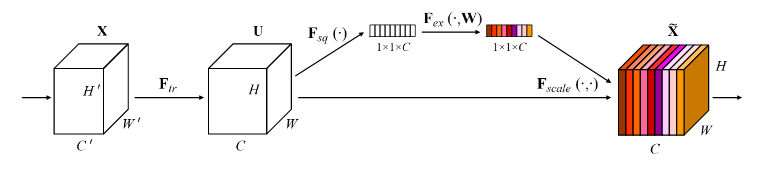
\includegraphics[width=0.8\textwidth]{background/se.png}
    \caption{}
    \label{figure:background:se}
\end{figure}

\subsection{Data Augmentation}

Image data augmentation is a set of techniques that aim at artificially augmenting the amount of data that can be obtained from the images in the dataset.  These techniques modify the images in the dataset creating new information that can be used as input for our model this way we can compensate for a small dataset obtaining a higher amount of information from the dataset. \\

Using data augmentation we can work with fewer images having a lower variance lowering the chances of overfitting and having a better understanding of the most important features of each class in the dataset. Variance can be defined as the tendency to learn random things irrespective of the real signal \cite{data_augmentation}.  Having a high variance implies that the model is learning from the noise of the data, in this case the model is overfitting. \\

DATA AUG + small samples

For data augmentation we will apply flipping, rotation and rescaling on our images.